\documentclass[11pt,a4paper]{article}
\usepackage[utf8]{inputenc}
\usepackage[T1]{fontenc}
\usepackage[spanish,es-nodecimaldot]{babel}
\usepackage{amsmath,amssymb,bm,booktabs,array,longtable,graphicx,geometry}
\usepackage[colorlinks=true,allcolors=blue]{hyperref}
\geometry{margin=24mm}
\newcommand{\PEB}{\operatorname{PEB}}
\graphicspath{{../Estimator comparisons/results/baseline_20260916_141449_280/figures_20260916_142555_600/}{../Estimator comparisons/results/receiver_order_20260916_141805_499/}{../Estimator comparisons/results/LED_calibration_20260916_141804_298/}}
\title{Estimadores para posicionamiento 3D con LED fijo y PD reorientable\\\large LS directo, GLS/WLS de cocientes y NLS conjunto con respuesta $\cos^{m_R}\psi$}
\author{Proyecto Cambridge}
\date{16 de septiembre de 2026}
\begin{document}
\maketitle
\begin{abstract}
Se implementan y contrastan cuatro estimadores de posición a partir de un barrido de normales conocidas de un único fotodiodo. La respuesta angular efectiva del receptor se generaliza a $\cos^{m_R}\psi$, con valor nominal $m_R=1$. Se demuestra que una etapa independiente de búsqueda de dirección seguida de otra estimación de distancia no es obligatoria: una parametrización óptica tridimensional permite LS directo y una única optimización NLS de las potencias originales. Los métodos GLS y WLS mantienen una arquitectura de dirección por cocientes y amplitud perfilada, pero con covarianzas derivadas para este modelo, sin copiar recortes de potencia de los códigos de referencia. Se evalúan error, sesgo empírico, fallos y distribuciones espaciales, y se analiza qué calibración es necesaria ante un LED cuasi-Lambertiano.
\end{abstract}
\tableofcontents
\clearpage

\section{Modelo y alcance de los algoritmos}
El LED está fijo en $\mathbf t$, con eje $\mathbf n_t$. El receptor permanece en la posición desconocida $\mathbf r$ mientras adopta normales conocidas $\mathbf n_i$. Se usan las definiciones:
\begin{equation}
 d=\|\mathbf t-\mathbf r\|,\quad \mathbf u=(\mathbf t-\mathbf r)/d,\quad
 \mathbf q=-\mathbf n_t,\quad c=\mathbf q^{\mathsf T}\mathbf u,\quad s_i=\mathbf n_i^{\mathsf T}\mathbf u.
\end{equation}
Con $\nu=m_R>0$ conocido y un patrón emisor calibrado $f_T(\mathbf u)>0$, el modelo en el interior visible es:
\begin{equation}
 \mu_i=\beta s_i^\nu,\qquad \beta=\frac{Cf_T(\mathbf u)}{d^2},\qquad
 \bar{\mathbf Y}\sim\mathcal N(\bm\mu,\Sigma),\quad \Sigma=\operatorname{diag}(\sigma^2/N_i).
\label{eq:model}
\end{equation}
Para un emisor Lambertiano, $f_T=c^{m_T}$ y $C=P_t(m_T+1)A_{\rm PD}T_sg/(2\pi)$. $m_R$ caracteriza la respuesta angular efectiva total, no la responsividad espectral en A/W, y no añade un factor $(m_R+1)$ a $C$. Si una medición de responsividad intrínseca excluye la proyección del área, debe incorporarse esa proyección antes de identificar el exponente efectivo del canal; no se debe contar dos veces el mismo coseno.

La cota generalizada y su demostración están en \path{../Bounds (3D)/Position Error Bound/PEB_derivation_mR.tex}; la derivación original se conserva intacta. Los ocho scripts de diseño usan $m_R=1$ por defecto y conservan sus funciones de dibujo. El parámetro se registra en los datos y en consola. Los MAT antiguos sin ese campo se interpretan como $m_R=1$.

\textbf{Alcance explícito de esta primera comparación:} los cuatro estimadores trabajan en una región de visibilidad completa, con $s_i>\cos\Psi$ y $c>0$. No se entrega una máscara verdadera al algoritmo. El simulador comprueba antes del Monte Carlo que la configuración seleccionada satisface esa hipótesis; si no, solicita cambiar FOV, orientaciones o región de evaluación. El NLS implementado resuelve esa rama física, no una búsqueda global entre todas las máscaras de un modelo de corte FOV discontinuo. No se utilizan límites de la rejilla como prior de posición, ni se conoce la altura del receptor durante la estimación.

\section{Una parametrización que evita dos estimaciones separadas}
Definimos el vector óptico:
\begin{equation}
 \mathbf v=\beta^{1/\nu}\mathbf u,\qquad \bm\mu^{\odot1/\nu}=H\mathbf v,
 \qquad H=\begin{bmatrix}\mathbf n_1^{\mathsf T}\\\vdots\\\mathbf n_K^{\mathsf T}\end{bmatrix}.
\label{eq:linear}
\end{equation}
La potencia y la raíz se aplican componente a componente. Si $H$ tiene rango tres, las potencias sin ruido determinan $\mathbf v$. La posición es una transformación algebraica:
\begin{equation}
 \mathbf r=\mathbf t-
 \sqrt{Cf_T\!\left(\frac{\mathbf v}{\|\mathbf v\|}\right)}\,
 \|\mathbf v\|^{-(\nu/2+1)}\mathbf v.
\label{eq:direct_position}
\end{equation}
Calcular una normalización y una raíz cuadrada en esta transformación no constituye una nueva etapa estadística: sólo convierte coordenadas. No requiere una adquisición adicional, realimentación al LED ni un segundo problema de búsqueda de dirección.

El Jacobiano de $\mathbf v$ respecto a $\mathbf r$ es invertible en el interior iluminado; para $a=\|\mathbf v\|$, su determinante es $2a^3/(\nu d^3)$. Como el Jacobiano de las potencias es $\nu\operatorname{diag}[(H\mathbf v)^{\nu-1}]H B_\nu$, se conserva la condición de rango de las normales. Tener $K\geq3$ es necesario, pero se necesita también diversidad lineal de las normales visibles.

\section{LS directo}
El estimador LS forma las raíces observadas y resuelve:
\begin{equation}
 \mathbf z=\bar{\mathbf Y}^{\odot1/\nu},\qquad
 \hat{\mathbf v}_{\rm LS}=\arg\min_{\mathbf v}\|H\mathbf v-\mathbf z\|^2
 =H^\dagger\mathbf z.
\end{equation}
La implementación usa una resolución por barra invertida, no la inversa explícita de $H^{\mathsf T}H$. Después aplica \eqref{eq:direct_position}. Es un ajuste conjunto de tres incógnitas.

Cuando $m_R=1$ y las varianzas son iguales, el modelo en $\mathbf v$ es exactamente lineal Gaussiano. Si la solución pertenece al dominio físico, LS es el MLE en esas coordenadas. Con varianzas diferentes, el MLE es el LS generalizado directo:
\begin{equation}
 \hat{\mathbf v}=(H^{\mathsf T}\Sigma^{-1}H)^{-1}H^{\mathsf T}\Sigma^{-1}\bar{\mathbf Y}.
\label{eq:direct_weighted}
\end{equation}
El NLS implementado utiliza esta solución exacta como caso especial de $m_R=1$. Por ello LS y NLS coinciden con muestras iguales; no se introduce una diferencia artificial para separar sus curvas.

Para $m_R\ne1$, transformar las observaciones transforma también el ruido. A primer orden:
\begin{equation}
 \Sigma_z\simeq D\Sigma D,\qquad
 D=\operatorname{diag}\left[\frac1\nu\mu_i^{1/\nu-1}\right].
\end{equation}
El ruido transformado es aproximadamente heteroscedástico y las raíces tienen sesgo de orden superior. LS no es entonces, en general, el MLE de las potencias originales. En el código se normaliza primero por una escala positiva de potencia para evitar potencias numéricas extremas; esa escala se conserva para reconstruir $\beta$ y la posición.

\section{GLS y WLS basados en cocientes}
Los algoritmos de referencia \cite{tcom,broadcast} motivan la cancelación de amplitud, pero el receptor reorientable exige utilizar $m_R$, no el orden emisor, en la transformación de cocientes.

Sea $j$ la referencia de mayor potencia observada y $t_i=z_i/z_j$ para $i\ne j$. El modelo sin ruido satisface:
\begin{equation}
 (\mathbf n_i-t_i\mathbf n_j)^{\mathsf T}\mathbf u=0,\qquad i\ne j.
\end{equation}
Escribimos $A=LH$, donde cada fila de $L$ tiene un uno en $i$ y $-t_i$ en $j$. La covarianza de los errores de cocientes, por linealización, es proporcional a:
\begin{equation}
 C_r=L\Sigma_zL^{\mathsf T}
 =\operatorname{diag}\{v_{z,i}:i\ne j\}+v_{z,j}\mathbf t\mathbf t^{\mathsf T}.
\label{eq:ratio_cov}
\end{equation}
Los factores escalares comunes asociados a $z_j$ y a la amplitud se cancelan del criterio de dirección. El término exterior conserva la correlación compartida por la referencia. Las varianzas $v_{z,i}$ se calculan con la derivada de la raíz y las varianzas $\sigma^2/N_i$, sustituyendo medias desconocidas por observaciones cuando la transformación es válida.

\subsection{GLS de cocientes}
La dirección es el autovector unitario de menor autovalor de:
\begin{equation}
 M_{\rm GLS}=A^{\mathsf T}C_r^{-1}A.
\end{equation}
Se usa Cholesky para blanquear $A$ y una descomposición simétrica $3\times3$. Se elige el signo físico y se comprueba visibilidad. Este GLS es una aproximación estadística de primer orden; no se afirma que sea el MLE exacto de cocientes ruidosos a cualquier SNR. La normalización y los pesos observados pueden producir términos de sesgo de orden superior.

\subsection{WLS de cocientes}
WLS conserva sólo la diagonal de \eqref{eq:ratio_cov}:
\begin{equation}
 M_{\rm WLS}=A^{\mathsf T}\operatorname{diag}(C_r)^{-1}A.
\end{equation}
Es más simple, pero ignora la correlación introducida por la referencia. No debe confundirse con un WLS directo óptimo en el dominio original: los nombres GLS/WLS de este informe designan específicamente estas variantes de cocientes. En ruido independiente, un GLS directo en las potencias de $m_R=1$ coincide con el WLS directo; crear nombres diferentes no crea información diferente.

\subsection{Amplitud y distancia sin una medición adicional}
Con la dirección estimada se forma $h_i=(\mathbf n_i^{\mathsf T}\hat{\mathbf u})^\nu$. El máximo de verosimilitud Gaussiano condicional en amplitud es:
\begin{equation}
 \hat\beta=\frac{\mathbf h^{\mathsf T}\Sigma^{-1}\bar{\mathbf Y}}
 {\mathbf h^{\mathsf T}\Sigma^{-1}\mathbf h},\qquad
 \hat d=\sqrt{\frac{Cf_T(\hat{\mathbf u})}{\hat\beta}},\qquad
 \hat{\mathbf r}=\mathbf t-\hat d\hat{\mathbf u}.
\label{eq:profile}
\end{equation}
Éste es el análogo dual de \texttt{broadcast\_distance}: el factor común ahora contiene irradiación del LED fijo, mientras que la respuesta del PD varía entre adquisiciones. Se utilizan las mismas $K$ potencias. Un numerador no positivo no se sustituye por una potencia artificial; se registra una estimación no física.

\section{NLS conjunto en las potencias originales}
El objetivo es:
\begin{equation}
 \hat{\mathbf v}_{\rm NLS}=\arg\min_{\mathbf v\in\mathcal D}
 \sum_i\frac{N_i}{\sigma^2}\left[(\mathbf n_i^{\mathsf T}\mathbf v)^\nu-\bar Y_i\right]^2,
\end{equation}
con dominio de visibilidad completa:
\begin{equation}
 \mathcal D=\{\mathbf v:\|\mathbf v\|>0,\ \mathbf q^{\mathsf T}\mathbf v>0,
 \ \mathbf n_i^{\mathsf T}\mathbf v>\|\mathbf v\|\cos\Psi,\ \mathbf n_i^{\mathsf T}\mathbf v>0\ \forall i\}.
\end{equation}
La transformación \eqref{eq:direct_position} es biyectiva en el dominio iluminado, así que optimizar en $\mathbf v$ equivale a una optimización conjunta de posición en esa rama. El Jacobiano analítico de la media es:
\begin{equation}
 \frac{\partial\mu_i}{\partial\mathbf v^{\mathsf T}}=
 \nu(\mathbf n_i^{\mathsf T}\mathbf v)^{\nu-1}\mathbf n_i^{\mathsf T}.
\end{equation}
Se implementa Levenberg--Marquardt con escalado diagonal, aceptación por disminución del objetivo y control del dominio. No requiere Optimization Toolbox. La inicialización es LS transformado cuando es válida; en otro caso se usa una dirección física conocida como semilla con amplitud perfilada. Usar una semilla no convierte el ajuste final en dos estimadores independientes. No se garantiza un mínimo global para $m_R\ne1$ o configuraciones de baja SNR.

NLS utiliza directamente potencias negativas producidas por ruido Gaussiano; no necesita obtener su raíz. Las variantes transformadas requieren potencias positivas para $m_R\ne1$ y declaran fallo si no se cumple. Para $m_R=1$, LS permite observaciones negativas, aunque la solución física final debe tener amplitud positiva y orientación admisible.

\section{Comparación con la cota y tratamiento de fallos}
Se genera una única matriz de potencias ruidosas para todos los métodos de cada ensayo. Las semillas se conservan y se restaura el estado del generador aleatorio al terminar. El PEB se evalúa con el modelo verdadero y las mismas muestras y normales, utilizando el gradiente cartesiano generalizado. No se suman cotas independientes de dirección y distancia ignorando sus correlaciones.

Los resultados guardan posiciones estimadas, errores, direcciones, amplitudes, objetivos, iteraciones, códigos de estado, observaciones y parámetros verdaderos/asumidos. Los fallos no desaparecen de los CDF: su masa queda en infinito. Se muestran RMSE de estimaciones válidas y tasa de fallos por separado. Por convención operativa, el RMSE completo vale infinito si falta alguna estimación; no se interpreta como un error físico medido infinito.

El CDF del error por ensayo no es un CDF del PEB. Se muestra aparte un CDF espacial de RMSE por posición y PEB, sobre las mismas posiciones. Para mantener la exportación vectorial manejable, el CDF gráfico puede muestrear hasta 2000 rangos ordenados; se guardan todos los datos y no se renormaliza la masa de fallos.

Los intervalos de Monte Carlo del RMSE se obtienen propagando la varianza de la media del error cuadrático, estratificada por posición. Son intervalos de incertidumbre de la simulación, no regiones de confianza de localización. El sesgo empírico obtenido promediando un número finito de ensayos contiene también incertidumbre Monte Carlo; no demuestra por sí solo un sesgo estructural pequeño.

\section{Resultados verificados}
La comparación nominal usa $P_t=0.65$ W, área $75.4\ \mathrm{mm}^2$, FOV $46^\circ$, LED a $(0,0,2.5)$ m, $\Phi_{1/2}=45^\circ$, $K=9$, cono de $10^\circ$, $N_i=1000$ y $\sigma^2=3\times10^{-14}\ \mathrm W^2$. Se selecciona explícitamente la región $x,y\in[-0.4,0.4]$ m y $z\in\{0.2,0.8,1.4\}$ m, donde todas las orientaciones son visibles. No representa el recinto completo con esa FOV. La primera simulación usa 75 posiciones y 500 ensayos por posición:
\begin{center}
\begin{tabular}{lrrr}
\toprule
Método & RMSE [cm] & RMSE/RMS-PEB & Fallos \\
\midrule
LS directo & 0.76511 & 1.01096 & 0\% \\
GLS de cocientes & 0.76514 & 1.01101 & 0\% \\
WLS de cocientes & 0.99314 & 1.31226 & 0\% \\
NLS conjunto & 0.76511 & 1.01096 & 0\% \\
\bottomrule
\end{tabular}
\end{center}
El RMS-PEB es 0.75681 cm. La coincidencia de LS y NLS es la esperada para $m_R=1$ y varianzas iguales. GLS es muy próximo en esta SNR. La diferencia de WLS es coherente con ignorar covarianzas de referencia. La proximidad a una cota local no demuestra insesgadez exacta ni eficiencia global a baja SNR.
\begin{figure}[htbp]\centering

\includegraphics[width=0.95\linewidth]{Estimator_RMSE_vs_3D_PEB.pdf}
\caption{Comparación nominal, $m_R=1$. Los intervalos cuantifican la incertidumbre Monte Carlo. El panel inferior hace explícitos los fallos.}
\end{figure}
\begin{figure}[htbp]\centering

\includegraphics[width=0.95\linewidth]{Estimator_error_CDF.pdf}
\caption{Distribución de errores euclídeos de todos los ensayos; la coincidencia de LS y NLS no es un error de dibujo.}
\end{figure}
\begin{figure}[htbp]\centering

\includegraphics[width=0.95\linewidth]{Estimator_spatial_RMSE_CDF.pdf}
\caption{Distribuciones espaciales de RMSE y PEB. No son distribuciones de una misma variable aleatoria por ensayo.}
\end{figure}

El barrido de orden usa 27 posiciones y 200 ensayos por punto. Con ruido nominal, los RMS-PEB para $m_R=0.5,1,2,3$ son aproximadamente $1.5189,0.7819,0.4164,0.2974$ cm, y NLS obtiene $1.5485,0.7969,0.4241,0.3026$ cm. El aumento de pendiente angular mejora la información en esta región central, pero no implica que órdenes mayores sean mejores a cualquier incidencia. $m_R$ es un parámetro físico a calibrar, no un hiperparámetro que deba ajustarse para reducir artificialmente una cota.
\begin{figure}[htbp]\centering
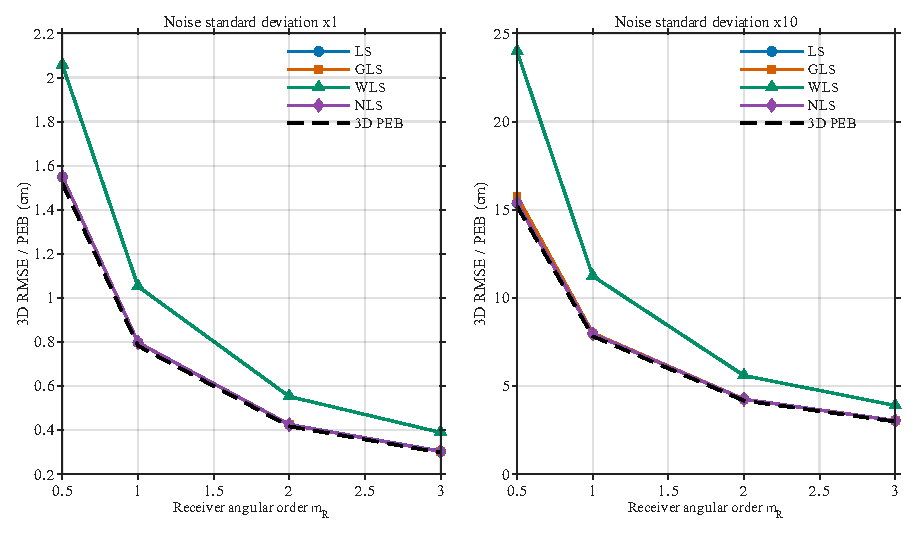
\includegraphics[width=0.95\linewidth]{Estimators_vs_receiver_order.pdf}
\caption{Orden receptor y ruido. Multiplicar por diez la desviación estándar multiplica por cien la varianza. Los casos de orden diferente comparan respuestas físicas diferentes a igual ganancia normal y ruido.}
\end{figure}

\section{Importancia del patrón de irradiación del LED}
Para un LED fijo y una posición estacionaria, $f_T(\mathbf u)$ es común a todas las orientaciones del PD. Por tanto, los cocientes cancelan ese factor y el ajuste en $\mathbf v$ tampoco necesita su forma angular. Esto permite estimar dirección sin utilizar el patrón emisor en la parte determinista del ajuste, siempre que $m_R$ y las normales se conozcan. La precisión sigue dependiendo indirectamente del patrón verdadero a través de la potencia recibida y la SNR.

La distancia sí necesita irradiancia angular absoluta calibrada. En ausencia de ruido, si el algoritmo utiliza un patrón y ganancia incorrectos:
\begin{equation}
 \frac{\hat d}{d}=\sqrt{\frac{C_{\rm asumido}f_{T,\rm asumido}(\mathbf u)}
 {C_{\rm real}f_{T,\rm real}(\mathbf u)}}.
\label{eq:pattern_bias}
\end{equation}
Ningún cambio de LS a NLS elimina esta ambigüedad física. Más muestras tampoco elimina un sesgo sistemático de calibración. Si se desconoce toda la escala óptica, $d\mapsto kd$, $C\mapsto k^2C$ conserva todas las potencias y la distancia no es identificable sin información adicional.

La prueba de desajuste usa un patrón cuasi-Lambertiano controlado:
\begin{equation}
 f_T(\mathbf u)=c^{m_T}\left[1+\epsilon\left((\mathbf e_1^{\mathsf T}\mathbf u)^2-(\mathbf e_2^{\mathsf T}\mathbf u)^2\right)\right],\quad |\epsilon|<1.
\end{equation}
Es positivo, conserva potencia total por promedio azimutal cero y coincide con la ganancia normal. No se presenta como ajuste de un LED comercial. Para $\epsilon=0.3$, NLS alcanza aproximadamente 1.3038 cm suponiendo un LED Lambertiano, frente a 0.7978 cm con el patrón calibrado y PEB de 0.7828 cm. La dirección estimada es idéntica para los mismos datos en ambas configuraciones de modelo; la diferencia se concentra en la recuperación de distancia.
\begin{figure}[htbp]\centering
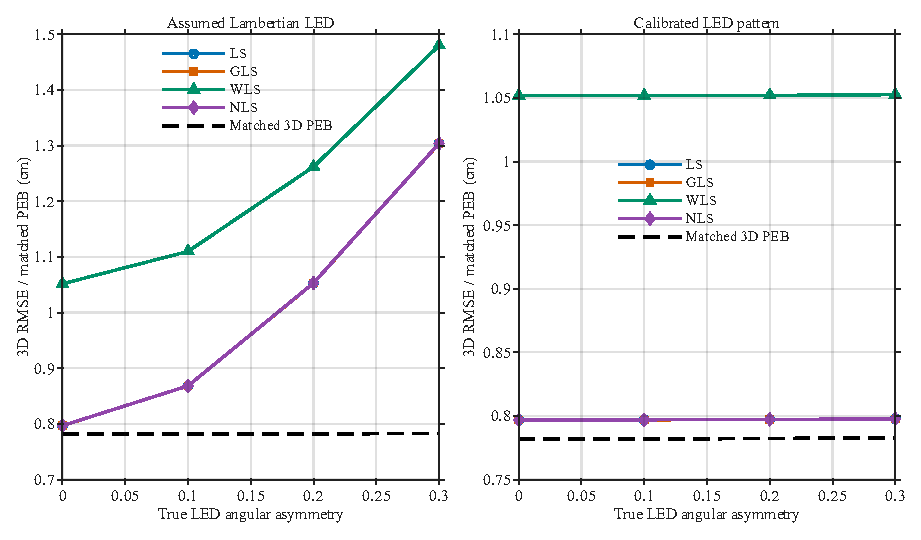
\includegraphics[width=0.95\linewidth]{LED_pattern_calibration.pdf}
\caption{Desajuste del patrón emisor. La curva PEB usa el modelo verdadero conocido y es una referencia optimista para algoritmos que lo desconocen, no una cota universal del MSE de un estimador sesgado por desajuste.}
\end{figure}

\section{Calibración necesaria}
\begin{enumerate}
\item \textbf{Geometría y sistema global.} Posición y eje del LED; transformaciones del soporte, del gimbal y de la IMU a coordenadas globales; ceros de inclinación y azimut; ortogonalidad, holgura y repetibilidad. Debe localizarse el centro óptico respecto al pivote para corregir traslaciones inducidas por giro.
\item \textbf{Respuesta del receptor.} Medir corriente o potencia frente a incidencia conocida manteniendo distancia e irradiación constantes. Ajustar la respuesta efectiva, $m_R$, FOV y posibles dependencias de azimut. Comprobar residuos fuera del ajuste: una única potencia de coseno no representa necesariamente filtros, encapsulado o lentes reales.
\item \textbf{Escala radiométrica de extremo a extremo.} Calibrar el producto efectivo de potencia emitida, área, transmisión, ganancia óptica, responsividad espectral y electrónica de lectura. Si se usan voltios o amperios, convertir consistentemente media y varianza al mismo dominio. Para luz blanca la responsividad efectiva depende del espectro; un valor nominal de 0.4 A/W no constituye por sí solo una calibración.
\item \textbf{Patrón emisor.} Medir intensidad frente a ángulo polar y azimut con geometría y receptor calibrados. Un ajuste Lambertiano puede bastar sólo si sus residuos son compatibles con el objetivo de distancia. Si no, usar un patrón medido/interpolado y sus derivadas para la cota. La referencia azimutal importa para patrones no simétricos.
\item \textbf{Fondo y deriva.} Medir oscuridad, offsets y luz ambiente; preferir extracción de una componente modulada identificable del LED. En $m_R=1$, un fondo común desconocido se confunde con la componente vertical de un cono de inclinación única. Vigilar deriva de potencia, temperatura y ganancia durante el barrido; si cambian con la orientación/tiempo, dejan de cancelarse como amplitud común.
\item \textbf{Ruido y muestras efectivas.} Estimar varianza, correlaciones temporales, saturación y linealidad. Con muestras correlacionadas, la varianza de la media es $N^{-2}\mathbf1^{\mathsf T}\Sigma_t\mathbf1$, no necesariamente $\sigma^2/N$. La capacitancia y el ruido de un PD mayor pueden invalidar el escalado ideal $1/A$.
\end{enumerate}
Si la covarianza del ruido depende de posición, la FIM Gaussiana necesita también el término de derivadas de covarianza. No es correcto sustituir una varianza dependiente de señal en una fórmula homoscedástica y omitirlo. Asimismo, parámetros de calibración inciertos deben añadirse como auxiliares o modelarse mediante una cota adecuada; el PEB nominal con parámetros perfectos no los incluye.

\section{Archivos, uso y límites de la comparación}
\begin{longtable}{>{\raggedright\arraybackslash}p{0.42\linewidth}>{\raggedright\arraybackslash}p{0.51\linewidth}}
\toprule Archivo & Función \\
\midrule\endhead
\path{Estimators/rx_estimate.m} & Interfaz común para matrices $K\times T$ de medias RSS, con estados de éxito/fallo y diagnósticos. \\
\path{rx_estimate_ls.m}, \path{rx_estimate_gls.m}, \path{rx_estimate_wls.m}, \path{rx_estimate_nls.m} & Entradas explícitas de los cuatro métodos. \\
\path{rx_optical_ls.m}, \path{rx_ratio_direction.m}, \path{rx_optical_nls.m} & Núcleos matemáticos independientes; no utilizan posiciones verdaderas. \\
\path{rx_profile_amplitude.m}, \path{rx_optical_position.m} & Amplitud condicional y conversión óptica a posición. \\
\path{Estimator comparisons/sim01_estimators_vs_PEB.m} & Comparación nominal y dos tipos de CDF. \\
\path{sim02_estimators_vs_mR.m} & Barrido controlado de respuesta receptora y ruido. \\
\path{sim03_LED_pattern_calibration.m} & Modelo emisor correcto frente a desajuste cuasi-Lambertiano. \\
\path{rx_monte_carlo.m}, \path{rx_mc_metrics.m} & Generación común de datos, estados, errores, sesgos empíricos y estadísticas. \\
\path{replot_estimator_results.m} & Regenera figuras desde MAT sin volver a estimar. \\
\bottomrule
\end{longtable}
Las funciones del núcleo de estimadores están en la primera carpeta y los scripts/estadísticas en la segunda. Los resultados usan carpetas con fecha, guardan todos los ensayos y no sobrescriben versiones previas. El escenario debe elegirse antes de comparar; la comprobación de visibilidad no selecciona a posteriori los ensayos favorables.

\begin{verbatim}
addpath('CAMBRIDGE/simulations');
cambridge_setup();
sim01_estimators_vs_PEB;
\end{verbatim}
Después de una ejecución puede cambiarse sólo el estilo y redibujar:
\begin{verbatim}
s = ieee_plot_style();
s.font_size = 9;
replot_estimator_results(fullfile(result.output_directory, ...
    'comparison_results.mat'), s);
\end{verbatim}

\section{Respuesta a la pregunta de una o dos etapas}
\textbf{No se requieren necesariamente dos etapas.} LS directo estima tres componentes ópticas simultáneamente y NLS ajusta conjuntamente esas mismas tres incógnitas a las potencias originales. La transformación final a coordenadas espaciales es algebraica. GLS/WLS de cocientes sí son alternativas de dirección y amplitud, útiles para contrastar estrategias, pero no una imposición física de la arquitectura.

\textbf{El patrón del LED es esencial para distancia, no para la forma determinista de la dirección.} Un LED cuasi-Lambertiano no invalida la arquitectura si su patrón se conoce y se calibra, pero utilizar un patrón incorrecto introduce el sesgo de \eqref{eq:pattern_bias}.

\textbf{La calibración es parte del sistema, no un ajuste opcional posterior.} Sin escala radiométrica o actitud global suficiente no se obtiene la misma identificabilidad de posición. Los resultados de este informe son de un modelo ideal calibrado. La sensibilidad a errores de reorientación se estudia posteriormente, en una carpeta separada y con una distinción explícita entre incertidumbre de medida de pose y perturbaciones de actuación.

\bibliographystyle{IEEEtran}
\bibliography{estimator_references}
\end{document}
